\documentclass{report}

%%%%%%%%%%%%%%%%%%%%%%%%%%%%%%%%%
% PACKAGE IMPORTS
%%%%%%%%%%%%%%%%%%%%%%%%%%%%%%%%%


\usepackage[tmargin=2cm,rmargin=1in,lmargin=1in,margin=0.85in,bmargin=2cm,footskip=.2in]{geometry}
\usepackage{amsmath,amsfonts,amsthm,amssymb,mathtools}
\usepackage{bookmark}
\usepackage{enumitem}
\usepackage{hyperref,theoremref}
\hypersetup{
	pdftitle={Assignment-1},
	colorlinks=true, linkcolor=doc!90,
	citecolor=doc!90,
	bookmarksnumbered=true,
	bookmarksopen=true
}
\usepackage[most,many,breakable]{tcolorbox}
\usepackage{xcolor}
\usepackage{varwidth}
\usepackage{varwidth}
\usepackage{etoolbox}
%\usepackage{authblk}
\usepackage{nameref}
\usepackage{multicol,array}
\usepackage{tikz-cd}
\usepackage{textcomp}
\usetikzlibrary {positioning}
\usepackage{gensymb}
%\usepackage{import}
%\usepackage{xifthen}
%\usepackage{pdfpages}
%\usepackage{transparent}


%%%%%%%%%%%%%%%%%%%%%%%%%%%%%%
% SELF MADE COLORS
%%%%%%%%%%%%%%%%%%%%%%%%%%%%%%



\definecolor{myg}{RGB}{56, 140, 70}
\definecolor{myb}{RGB}{45, 111, 177}
\definecolor{myr}{RGB}{199, 68, 64}
\definecolor{mym}{RGB}{0, 93, 93}
\definecolor{mytheorembg}{HTML}{F2F2F9}
\definecolor{mytheoremfr}{HTML}{00007B}
\definecolor{myexamplebg}{HTML}{F2FBF8}
\definecolor{myexamplefr}{HTML}{88D6D1}
\definecolor{myexampleti}{HTML}{2A7F7F}
\definecolor{mydefinitbg}{HTML}{E5E5FF}
\definecolor{mydefinitfr}{HTML}{3F3FA3}
\definecolor{notesgreen}{RGB}{0,162,0}
\definecolor{myp}{RGB}{197, 92, 212}
\definecolor{mygr}{HTML}{2C3338}
\definecolor{myred}{RGB}{127,0,0}
\definecolor{myyellow}{RGB}{169,121,69}
\definecolor{processblue}{cmyk}{0.96,0,0,0}

%%%%%%%%%%%%%%%%%%%%%%%%%%%%
% TCOLORBOX SETUPS
%%%%%%%%%%%%%%%%%%%%%%%%%%%%

\setlength{\parindent}{1cm}
%================================
% THEOREM BOX
%================================

\tcbuselibrary{theorems,skins,hooks}
\newtcbtheorem[number within=section]{Theorem}{Theorem}
{%
	enhanced,
	breakable,
	colback = mytheorembg,
	frame hidden,
	boxrule = 0sp,
	borderline west = {2pt}{0pt}{mytheoremfr},
	sharp corners,
	detach title,
	before upper = \tcbtitle\par\smallskip,
	coltitle = mytheoremfr,
	fonttitle = \bfseries\sffamily,
	description font = \mdseries,
	separator sign none,
	segmentation style={solid, mytheoremfr},
}
{th}

\tcbuselibrary{theorems,skins,hooks}
\newtcbtheorem[number within=chapter]{theorem}{Theorem}
{%
	enhanced,
	breakable,
	colback = mytheorembg,
	frame hidden,
	boxrule = 0sp,
	borderline west = {2pt}{0pt}{mytheoremfr},
	sharp corners,
	detach title,
	before upper = \tcbtitle\par\smallskip,
	coltitle = mytheoremfr,
	fonttitle = \bfseries\sffamily,
	description font = \mdseries,
	separator sign none,
	segmentation style={solid, mytheoremfr},
}
{th}


\tcbuselibrary{theorems,skins,hooks}
\newtcolorbox{Theoremcon}
{%
	enhanced
	,breakable
	,colback = mytheorembg
	,frame hidden
	,boxrule = 0sp
	,borderline west = {2pt}{0pt}{mytheoremfr}
	,sharp corners
	,description font = \mdseries
	,separator sign none
}


%================================
% Corollery
%================================
\tcbuselibrary{theorems,skins,hooks}
\newtcbtheorem[number within=section]{corolary}{Corollary}
{%
	enhanced
	,breakable
	,colback = myp!10
	,frame hidden
	,boxrule = 0sp
	,borderline west = {2pt}{0pt}{myp!85!black}
	,sharp corners
	,detach title
	,before upper = \tcbtitle\par\smallskip
	,coltitle = myp!85!black
	,fonttitle = \bfseries\sffamily
	,description font = \mdseries
	,separator sign none
	,segmentation style={solid, myp!85!black}
}
{th}
\tcbuselibrary{theorems,skins,hooks}
\newtcbtheorem[number within=chapter]{corollary}{Corollary}
{%
	enhanced
	,breakable
	,colback = myp!10
	,frame hidden
	,boxrule = 0sp
	,borderline west = {2pt}{0pt}{myp!85!black}
	,sharp corners
	,detach title
	,before upper = \tcbtitle\par\smallskip
	,coltitle = myp!85!black
	,fonttitle = \bfseries\sffamily
	,description font = \mdseries
	,separator sign none
	,segmentation style={solid, myp!85!black}
}
{th}

%================================
% CLAIM
%================================

\tcbuselibrary{theorems,skins,hooks}
\newtcbtheorem[number within=section]{claim}{Claim}
{%
	enhanced
	,breakable
	,colback = myg!10
	,frame hidden
	,boxrule = 0sp
	,borderline west = {2pt}{0pt}{myg}
	,sharp corners
	,detach title
	,before upper = \tcbtitle\par\smallskip
	,coltitle = myg!85!black
	,fonttitle = \bfseries\sffamily
	,description font = \mdseries
	,separator sign none
	,segmentation style={solid, myg!85!black}
}
{th}


%================================
% CONJECTURE
%================================

\tcbuselibrary{theorems,skins,hooks}
\newtcbtheorem[number within=section]{conjecture}{Conjecture}
{%
	enhanced
	,breakable
	,colback = mym!10
	,frame hidden
	,boxrule = 0sp
	,borderline west = {2pt}{0pt}{mym}
	,sharp corners
	,detach title
	,before upper = \tcbtitle\par\smallskip
	,coltitle = mym!85!black
	,fonttitle = \bfseries\sffamily
	,description font = \mdseries
	,separator sign none
	,segmentation style={solid, mym!85!black}
}
{th}

%================================
% EXAMPLE BOX
%================================

\newtcbtheorem[number within=section]{Example}{Example}
{%
	colback = myexamplebg
	,breakable
	,colframe = myexamplefr
	,coltitle = myexampleti
	,boxrule = 1pt
	,sharp corners
	,detach title
	,before upper=\tcbtitle\par\smallskip
	,fonttitle = \bfseries
	,description font = \mdseries
	,separator sign none
	,description delimiters parenthesis
}
{ex}

\newtcbtheorem[number within=chapter]{example}{Example}
{%
	colback = myexamplebg
	,breakable
	,colframe = myexamplefr
	,coltitle = myexampleti
	,boxrule = 1pt
	,sharp corners
	,detach title
	,before upper=\tcbtitle\par\smallskip
	,fonttitle = \bfseries
	,description font = \mdseries
	,separator sign none
	,description delimiters parenthesis
}
{ex}

%================================
% DEFINITION BOX
%================================

\newtcbtheorem[number within=section]{Definition}{Definition}{enhanced,
	before skip=2mm,after skip=2mm, colback=red!5,colframe=red!80!black,boxrule=0.5mm,
	attach boxed title to top left={xshift=1cm,yshift*=1mm-\tcboxedtitleheight}, varwidth boxed title*=-3cm,
	boxed title style={frame code={
					\path[fill=tcbcolback]
					([yshift=-1mm,xshift=-1mm]frame.north west)
					arc[start angle=0,end angle=180,radius=1mm]
					([yshift=-1mm,xshift=1mm]frame.north east)
					arc[start angle=180,end angle=0,radius=1mm];
					\path[left color=tcbcolback!60!black,right color=tcbcolback!60!black,
						middle color=tcbcolback!80!black]
					([xshift=-2mm]frame.north west) -- ([xshift=2mm]frame.north east)
					[rounded corners=1mm]-- ([xshift=1mm,yshift=-1mm]frame.north east)
					-- (frame.south east) -- (frame.south west)
					-- ([xshift=-1mm,yshift=-1mm]frame.north west)
					[sharp corners]-- cycle;
				},interior engine=empty,
		},
	fonttitle=\bfseries,
	title={#2},#1}{def}
\newtcbtheorem[number within=chapter]{definition}{Definition}{enhanced,
	before skip=2mm,after skip=2mm, colback=red!5,colframe=red!80!black,boxrule=0.5mm,
	attach boxed title to top left={xshift=1cm,yshift*=1mm-\tcboxedtitleheight}, varwidth boxed title*=-3cm,
	boxed title style={frame code={
					\path[fill=tcbcolback]
					([yshift=-1mm,xshift=-1mm]frame.north west)
					arc[start angle=0,end angle=180,radius=1mm]
					([yshift=-1mm,xshift=1mm]frame.north east)
					arc[start angle=180,end angle=0,radius=1mm];
					\path[left color=tcbcolback!60!black,right color=tcbcolback!60!black,
						middle color=tcbcolback!80!black]
					([xshift=-2mm]frame.north west) -- ([xshift=2mm]frame.north east)
					[rounded corners=1mm]-- ([xshift=1mm,yshift=-1mm]frame.north east)
					-- (frame.south east) -- (frame.south west)
					-- ([xshift=-1mm,yshift=-1mm]frame.north west)
					[sharp corners]-- cycle;
				},interior engine=empty,
		},
	fonttitle=\bfseries,
	title={#2},#1}{def}



%================================
% EXERCISE BOX
%================================

\makeatletter
\newtcbtheorem{question}{Question}{enhanced,
	breakable,
	colback=white,
	colframe=myb!80!black,
	attach boxed title to top left={yshift*=-\tcboxedtitleheight},
	fonttitle=\bfseries,
	title={#2},
	boxed title size=title,
	boxed title style={%
			sharp corners,
			rounded corners=northwest,
			colback=tcbcolframe,
			boxrule=0pt,
		},
	underlay boxed title={%
			\path[fill=tcbcolframe] (title.south west)--(title.south east)
			to[out=0, in=180] ([xshift=5mm]title.east)--
			(title.center-|frame.east)
			[rounded corners=\kvtcb@arc] |-
			(frame.north) -| cycle;
		},
	#1
}{def}
\makeatother

%================================
% SOLUTION BOX
%================================

\makeatletter
\newtcolorbox{solution}{enhanced,
	breakable,
	colback=white,
	colframe=myg!80!black,
	attach boxed title to top left={yshift*=-\tcboxedtitleheight},
	title=Solution,
	boxed title size=title,
	boxed title style={%
			sharp corners,
			rounded corners=northwest,
			colback=tcbcolframe,
			boxrule=0pt,
		},
	underlay boxed title={%
			\path[fill=tcbcolframe] (title.south west)--(title.south east)
			to[out=0, in=180] ([xshift=5mm]title.east)--
			(title.center-|frame.east)
			[rounded corners=\kvtcb@arc] |-
			(frame.north) -| cycle;
		},
}
\makeatother

%================================
% Question BOX
%================================

\makeatletter
\newtcbtheorem{qstion}{Question}{enhanced,
	breakable,
	colback=white,
	colframe=mygr,
	attach boxed title to top left={yshift*=-\tcboxedtitleheight},
	fonttitle=\bfseries,
	title={#2},
	boxed title size=title,
	boxed title style={%
			sharp corners,
			rounded corners=northwest,
			colback=tcbcolframe,
			boxrule=0pt,
		},
	underlay boxed title={%
			\path[fill=tcbcolframe] (title.south west)--(title.south east)
			to[out=0, in=180] ([xshift=5mm]title.east)--
			(title.center-|frame.east)
			[rounded corners=\kvtcb@arc] |-
			(frame.north) -| cycle;
		},
	#1
}{def}
\makeatother

\newtcbtheorem[number within=chapter]{wconc}{Wrong Concept}{
	breakable,
	enhanced,
	colback=white,
	colframe=myr,
	arc=0pt,
	outer arc=0pt,
	fonttitle=\bfseries\sffamily\large,
	colbacktitle=myr,
	attach boxed title to top left={},
	boxed title style={
			enhanced,
			skin=enhancedfirst jigsaw,
			arc=3pt,
			bottom=0pt,
			interior style={fill=myr}
		},
	#1
}{def}



%================================
% NOTE BOX
%================================

\usetikzlibrary{arrows,calc,shadows.blur}
\tcbuselibrary{skins}
\newtcolorbox{note}[1][]{%
	enhanced jigsaw,
	colback=gray!20!white,%
	colframe=gray!80!black,
	size=small,
	boxrule=1pt,
	title=\textbf{Note:-},
	halign title=flush center,
	coltitle=black,
	breakable,
	drop shadow=black!50!white,
	attach boxed title to top left={xshift=1cm,yshift=-\tcboxedtitleheight/2,yshifttext=-\tcboxedtitleheight/2},
	minipage boxed title=1.5cm,
	boxed title style={%
			colback=white,
			size=fbox,
			boxrule=1pt,
			boxsep=2pt,
			underlay={%
					\coordinate (dotA) at ($(interior.west) + (-0.5pt,0)$);
					\coordinate (dotB) at ($(interior.east) + (0.5pt,0)$);
					\begin{scope}
						\clip (interior.north west) rectangle ([xshift=3ex]interior.east);
						\filldraw [white, blur shadow={shadow opacity=60, shadow yshift=-.75ex}, rounded corners=2pt] (interior.north west) rectangle (interior.south east);
					\end{scope}
					\begin{scope}[gray!80!black]
						\fill (dotA) circle (2pt);
						\fill (dotB) circle (2pt);
					\end{scope}
				},
		},
	#1,
}

\tcbuselibrary{skins}
\usetikzlibrary{shadings}
\newcounter{example}
\colorlet{colexam}{red!75!black}
\tcbset{
	base/.style={
		empty,
		frame engine=path,
		colframe=yellow!10,
		sharp corners,
		title={Example \thetcbcounter},
		attach boxed title to top left={yshift*=-\tcboxedtitleheight},
		boxed title style={size=minimal, top=4pt, left=4pt},
		coltitle=colexam,fonttitle=\large\bfseries\sffamily,
	}
}
\newtcolorbox[use counter=example]{myexamplec}{%
	base,
	drop fuzzy shadow,
	coltitle=black,
	borderline west={3pt}{-3pt}{teal!50},
	attach boxed title to top left={xshift=-3mm, yshift*=-\tcboxedtitleheight/2},
	boxed title style={right=3pt, bottom=3pt, overlay={
			\draw[draw=teal!70, fill=teal!70, line join=round]
			(frame.south west) -- (frame.north west) -- (frame.north east) --
			(frame.south east) -- ++(-2pt, 0) -- ++(-2pt, -4pt) --
			++(-2pt, 4pt) -- cycle;
	}},
	overlay unbroken={
		\scoped \shade[left color=teal!10!black, right color=teal]
		([yshift=-0.2pt]title.south west) -- ([xshift=-1.5pt, yshift=-0.2pt]title.south-|frame.west) -- ++(0, -6pt) -- cycle;
	},
}

%%%%%%%%%%%%%%%%%%%%%%%%%%%%%%
% SELF MADE COMMANDS
%%%%%%%%%%%%%%%%%%%%%%%%%%%%%%


\newcommand{\thm}[2]{\begin{Theorem}{#1}{}#2\end{Theorem}}
\newcommand{\cor}[2]{\begin{corolary}{#1}{}#2\end{corolary}}
\newcommand{\clm}[3]{\begin{claim}{#1}{#2}#3\end{claim}}
\newcommand{\wc}[2]{\begin{wconc}{#1}{}\setlength{\parindent}{1cm}#2\end{wconc}}
\newcommand{\thmcon}[1]{\begin{Theoremcon}{#1}\end{Theoremcon}}
\newcommand{\ex}[2]{\begin{Example}{#1}{}#2\end{Example}}
\newcommand{\dfn}[2]{\begin{Definition}[colbacktitle=red!75!black]{#1}{}#2\end{Definition}}
\newcommand{\dfnc}[2]{\begin{definition}[colbacktitle=red!75!black]{#1}{}#2\end{definition}}
\newcommand{\qs}[2]{\begin{question}{#1}{}#2\end{question}}
\newcommand{\pf}[2]{\begin{myproof}[#1]#2\end{myproof}}
\newcommand{\nt}[1]{\begin{note}#1\end{note}}

\newcommand*\circled[1]{\tikz[baseline=(char.base)]{
		\node[shape=circle,draw,inner sep=1pt] (char) {#1};}}
\newcommand\getcurrentref[1]{%
	\ifnumequal{\value{#1}}{0}
	{??}
	{\the\value{#1}}%
}
\newcommand{\getCurrentSectionNumber}{\getcurrentref{section}}
\newenvironment{myproof}[1][\proofname]{%
	\proof[\bfseries #1: ]%
}{\endproof}
\newcounter{mylabelcounter}

\makeatletter
\newcommand{\setword}[2]{%
	\phantomsection
	#1\def\@currentlabel{\unexpanded{#1}}\label{#2}%
}
\makeatother

\newcommand{\circuitdraw}[1]{\begin{center}
		\begin{tikzpicture}[-latex ,auto ,node distance =1 cm and 1cm ,on grid ,
	semithick ,
	state/.style ={ circle ,top color =white , bottom color = processblue!20 ,
		draw,processblue , text=blue , minimum width =1 mm}]
	#1
\end{tikzpicture}
\end{center}}


\tikzset{
	symbol/.style={
			draw=none,
			every to/.append style={
					edge node={node [sloped, allow upside down, auto=false]{$#1$}}}
		}
}

%\usepackage{framed}
%\usepackage{titletoc}
%\usepackage{etoolbox}
%\usepackage{lmodern}


%\patchcmd{\tableofcontents}{\contentsname}{\sffamily\contentsname}{}{}

%\renewenvironment{leftbar}
%{\def\FrameCommand{\hspace{6em}%
%		{\color{myyellow}\vrule width 2pt depth 6pt}\hspace{1em}}%
%	\MakeFramed{\parshape 1 0cm \dimexpr\textwidth-6em\relax\FrameRestore}\vskip2pt%
%}
%{\endMakeFramed}

%\titlecontents{chapter}
%[0em]{\vspace*{2\baselineskip}}
%{\parbox{4.5em}{%
%		\hfill\Huge\sffamily\bfseries\color{myred}\thecontentspage}%
%	\vspace*{-2.3\baselineskip}\leftbar\textsc{\small\chaptername~\thecontentslabel}\\\sffamily}
%{}{\endleftbar}
%\titlecontents{section}
%[8.4em]
%{\sffamily\contentslabel{3em}}{}{}
%{\hspace{0.5em}\nobreak\itshape\color{myred}\contentspage}
%\titlecontents{subsection}
%[8.4em]
%{\sffamily\contentslabel{3em}}{}{}  
%{\hspace{0.5em}\nobreak\itshape\color{myred}\contentspage}



%%%%%%%%%%%%%%%%%%%%%%%%%%%%%%%%%%%%%%%%%%%
% TABLE OF CONTENTS
%%%%%%%%%%%%%%%%%%%%%%%%%%%%%%%%%%%%%%%%%%%

\usepackage{tikz}
\definecolor{doc}{RGB}{0,60,110}
\usepackage{titletoc}
\contentsmargin{0cm}
\titlecontents{chapter}[3.7pc]
{\addvspace{30pt}%
	\begin{tikzpicture}[remember picture, overlay]%
		\draw[fill=doc!60,draw=doc!60] (-7,-.1) rectangle (-0.9,.5);%
		\pgftext[left,x=-3.5cm,y=0.2cm]{\color{white}\Large\sc\bfseries Chapter\ \thecontentslabel};%
	\end{tikzpicture}\color{doc!60}\large\sc\bfseries}%
{}
{}
{\;\titlerule\;\large\sc\bfseries Page \thecontentspage
	\begin{tikzpicture}[remember picture, overlay]
		\draw[fill=doc!60,draw=doc!60] (2pt,0) rectangle (4,0.1pt);
	\end{tikzpicture}}%
\titlecontents{section}[3.7pc]
{\addvspace{2pt}}
{\contentslabel[\thecontentslabel]{2pc}}
{}
{\hfill\small \thecontentspage}
[]
\titlecontents*{subsection}[3.7pc]
{\addvspace{-1pt}\small}
{}
{}
{\ --- \small\thecontentspage}
[ \textbullet\ ][]

\makeatletter
\renewcommand{\tableofcontents}{%
	\chapter*{%
	  \vspace*{-20\p@}%
	  \begin{tikzpicture}[remember picture, overlay]%
		  \pgftext[right,x=15cm,y=0.2cm]{\color{doc!60}\Huge\sc\bfseries \contentsname};%
		  \draw[fill=doc!60,draw=doc!60] (13,-.75) rectangle (20,1);%
		  \clip (13,-.75) rectangle (20,1);
		  \pgftext[right,x=15cm,y=0.2cm]{\color{white}\Huge\sc\bfseries \contentsname};%
	  \end{tikzpicture}}%
	\@starttoc{toc}}
\makeatother

\newcommand{\pd}[2]{\frac{\partial{#1}}{\partial{#2}}}
\newcommand{\pdd}[3]{\frac{\partial^#1{#2}}{\partial{#3}^#1}}
\newcommand{\pdm}[6]{\frac{\partial^#1{#2}}{\partial{#4}^#3 \partial{#6}^#5}}
\newcommand{\eps}{\epsilon}
\newcommand{\veps}{\varepsilon}
\newcommand{\Qed}{\begin{flushright}\qed\end{flushright}}
\newcommand{\parinn}{\setlength{\parindent}{1cm}}
\newcommand{\parinf}{\setlength{\parindent}{0cm}}
\newcommand{\norm}{\|\cdot\|}
\newcommand{\inorm}{\norm_{\infty}}
\newcommand{\opensets}{\{V_{\alpha}\}_{\alpha\in I}}
\newcommand{\oset}{V_{\alpha}}
\newcommand{\opset}[1]{V_{\alpha_{#1}}}
\newcommand{\lub}{\text{lub}}
\newcommand{\del}[2]{\frac{\partial #1}{\partial #2}}
\newcommand{\Del}[3]{\frac{\partial^{#1} #2}{\partial^{#1} #3}}
\newcommand{\deld}[2]{\dfrac{\partial #1}{\partial #2}}
\newcommand{\Deld}[3]{\dfrac{\partial^{#1} #2}{\partial^{#1} #3}}
\newcommand{\lm}{\lambda}
\newcommand{\uin}{\mathbin{\rotatebox[origin=c]{90}{$\in$}}}
\newcommand{\ueq}{\mathbin{\rotatebox[origin=c]{90}{$=$}}}
\newcommand{\usubset}{\mathbin{\rotatebox[origin=c]{90}{$\subset$}}}
\newcommand{\lt}{\left}
\newcommand{\rt}{\right}
\newcommand{\bs}[1]{\boldsymbol{#1}}
\newcommand{\exs}{\exists}
\newcommand{\st}{\strut}
\newcommand{\dps}[1]{\displaystyle{#1}}

\newcommand{\sol}{\setlength{\parindent}{0cm}\textbf{\textit{Solution:}}\setlength{\parindent}{1cm} }
\newcommand{\solve}[1]{\setlength{\parindent}{0cm}\textbf{\textit{Solution: }}\setlength{\parindent}{1cm}#1 \Qed}
\DeclareRobustCommand{\rchi}{{\mathpalette\irchi\relax}}
\newcommand{\irchi}[2]{\raisebox{\depth}{$#1\chi$}}

\newcommand{\starx}{\textasteriskcentered}
\newcommand{\dnt}{\coloneqq}
\newcommand{\coef}{\bbF[\overline{x}]}
\newcommand{\per}{\text{per}}
%---------------------------------------
% BlackBoard Math Fonts :-
%---------------------------------------

%Captital Letters
\newcommand{\bbA}{\mathbb{A}}	\newcommand{\bbB}{\mathbb{B}}
\newcommand{\bbC}{\mathbb{C}}	\newcommand{\bbD}{\mathbb{D}}
\newcommand{\bbE}{\mathbb{E}}	\newcommand{\bbF}{\mathbb{F}}
\newcommand{\bbG}{\mathbb{G}}	\newcommand{\bbH}{\mathbb{H}}
\newcommand{\bbI}{\mathbb{I}}	\newcommand{\bbJ}{\mathbb{J}}
\newcommand{\bbK}{\mathbb{K}}	\newcommand{\bbL}{\mathbb{L}}
\newcommand{\bbM}{\mathbb{M}}	\newcommand{\bbN}{\mathbb{N}}
\newcommand{\bbO}{\mathbb{O}}	\newcommand{\bbP}{\mathbb{P}}
\newcommand{\bbQ}{\mathbb{Q}}	\newcommand{\bbR}{\mathbb{R}}
\newcommand{\bbS}{\mathbb{S}}	\newcommand{\bbT}{\mathbb{T}}
\newcommand{\bbU}{\mathbb{U}}	\newcommand{\bbV}{\mathbb{V}}
\newcommand{\bbW}{\mathbb{W}}	\newcommand{\bbX}{\mathbb{X}}
\newcommand{\bbY}{\mathbb{Y}}	\newcommand{\bbZ}{\mathbb{Z}}

%---------------------------------------
% MathCal Fonts :-
%---------------------------------------

%Captital Letters
\newcommand{\mcA}{\mathcal{A}}	\newcommand{\mcB}{\mathcal{B}}
\newcommand{\mcC}{\mathcal{C}}	\newcommand{\mcD}{\mathcal{D}}
\newcommand{\mcE}{\mathcal{E}}	\newcommand{\mcF}{\mathcal{F}}
\newcommand{\mcG}{\mathcal{G}}	\newcommand{\mcH}{\mathcal{H}}
\newcommand{\mcI}{\mathcal{I}}	\newcommand{\mcJ}{\mathcal{J}}
\newcommand{\mcK}{\mathcal{K}}	\newcommand{\mcL}{\mathcal{L}}
\newcommand{\mcM}{\mathcal{M}}	\newcommand{\mcN}{\mathcal{N}}
\newcommand{\mcO}{\mathcal{O}}	\newcommand{\mcP}{\mathcal{P}}
\newcommand{\mcQ}{\mathcal{Q}}	\newcommand{\mcR}{\mathcal{R}}
\newcommand{\mcS}{\mathcal{S}}	\newcommand{\mcT}{\mathcal{T}}
\newcommand{\mcU}{\mathcal{U}}	\newcommand{\mcV}{\mathcal{V}}
\newcommand{\mcW}{\mathcal{W}}	\newcommand{\mcX}{\mathcal{X}}
\newcommand{\mcY}{\mathcal{Y}}	\newcommand{\mcZ}{\mathcal{Z}}



%---------------------------------------
% Bold Math Fonts :-
%---------------------------------------

%Captital Letters
\newcommand{\bmA}{\boldsymbol{A}}	\newcommand{\bmB}{\boldsymbol{B}}
\newcommand{\bmC}{\boldsymbol{C}}	\newcommand{\bmD}{\boldsymbol{D}}
\newcommand{\bmE}{\boldsymbol{E}}	\newcommand{\bmF}{\boldsymbol{F}}
\newcommand{\bmG}{\boldsymbol{G}}	\newcommand{\bmH}{\boldsymbol{H}}
\newcommand{\bmI}{\boldsymbol{I}}	\newcommand{\bmJ}{\boldsymbol{J}}
\newcommand{\bmK}{\boldsymbol{K}}	\newcommand{\bmL}{\boldsymbol{L}}
\newcommand{\bmM}{\boldsymbol{M}}	\newcommand{\bmN}{\boldsymbol{N}}
\newcommand{\bmO}{\boldsymbol{O}}	\newcommand{\bmP}{\boldsymbol{P}}
\newcommand{\bmQ}{\boldsymbol{Q}}	\newcommand{\bmR}{\boldsymbol{R}}
\newcommand{\bmS}{\boldsymbol{S}}	\newcommand{\bmT}{\boldsymbol{T}}
\newcommand{\bmU}{\boldsymbol{U}}	\newcommand{\bmV}{\boldsymbol{V}}
\newcommand{\bmW}{\boldsymbol{W}}	\newcommand{\bmX}{\boldsymbol{X}}
\newcommand{\bmY}{\boldsymbol{Y}}	\newcommand{\bmZ}{\boldsymbol{Z}}
%Small Letters
\newcommand{\bma}{\boldsymbol{a}}	\newcommand{\bmb}{\boldsymbol{b}}
\newcommand{\bmc}{\boldsymbol{c}}	\newcommand{\bmd}{\boldsymbol{d}}
\newcommand{\bme}{\boldsymbol{e}}	\newcommand{\bmf}{\boldsymbol{f}}
\newcommand{\bmg}{\boldsymbol{g}}	\newcommand{\bmh}{\boldsymbol{h}}
\newcommand{\bmi}{\boldsymbol{i}}	\newcommand{\bmj}{\boldsymbol{j}}
\newcommand{\bmk}{\boldsymbol{k}}	\newcommand{\bml}{\boldsymbol{l}}
\newcommand{\bmm}{\boldsymbol{m}}	\newcommand{\bmn}{\boldsymbol{n}}
\newcommand{\bmo}{\boldsymbol{o}}	\newcommand{\bmp}{\boldsymbol{p}}
\newcommand{\bmq}{\boldsymbol{q}}	\newcommand{\bmr}{\boldsymbol{r}}
\newcommand{\bms}{\boldsymbol{s}}	\newcommand{\bmt}{\boldsymbol{t}}
\newcommand{\bmu}{\boldsymbol{u}}	\newcommand{\bmv}{\boldsymbol{v}}
\newcommand{\bmw}{\boldsymbol{w}}	\newcommand{\bmx}{\boldsymbol{x}}
\newcommand{\bmy}{\boldsymbol{y}}	\newcommand{\bmz}{\boldsymbol{z}}

%---------------------------------------
% Scr Math Fonts :-
%---------------------------------------

\newcommand{\sA}{{\mathscr{A}}}   \newcommand{\sB}{{\mathscr{B}}}
\newcommand{\sC}{{\mathscr{C}}}   \newcommand{\sD}{{\mathscr{D}}}
\newcommand{\sE}{{\mathscr{E}}}   \newcommand{\sF}{{\mathscr{F}}}
\newcommand{\sG}{{\mathscr{G}}}   \newcommand{\sH}{{\mathscr{H}}}
\newcommand{\sI}{{\mathscr{I}}}   \newcommand{\sJ}{{\mathscr{J}}}
\newcommand{\sK}{{\mathscr{K}}}   \newcommand{\sL}{{\mathscr{L}}}
\newcommand{\sM}{{\mathscr{M}}}   \newcommand{\sN}{{\mathscr{N}}}
\newcommand{\sO}{{\mathscr{O}}}   \newcommand{\sP}{{\mathscr{P}}}
\newcommand{\sQ}{{\mathscr{Q}}}   \newcommand{\sR}{{\mathscr{R}}}
\newcommand{\sS}{{\mathscr{S}}}   \newcommand{\sT}{{\mathscr{T}}}
\newcommand{\sU}{{\mathscr{U}}}   \newcommand{\sV}{{\mathscr{V}}}
\newcommand{\sW}{{\mathscr{W}}}   \newcommand{\sX}{{\mathscr{X}}}
\newcommand{\sY}{{\mathscr{Y}}}   \newcommand{\sZ}{{\mathscr{Z}}}


%---------------------------------------
% Math Fraktur Font
%---------------------------------------

%Captital Letters
\newcommand{\mfA}{\mathfrak{A}}	\newcommand{\mfB}{\mathfrak{B}}
\newcommand{\mfC}{\mathfrak{C}}	\newcommand{\mfD}{\mathfrak{D}}
\newcommand{\mfE}{\mathfrak{E}}	\newcommand{\mfF}{\mathfrak{F}}
\newcommand{\mfG}{\mathfrak{G}}	\newcommand{\mfH}{\mathfrak{H}}
\newcommand{\mfI}{\mathfrak{I}}	\newcommand{\mfJ}{\mathfrak{J}}
\newcommand{\mfK}{\mathfrak{K}}	\newcommand{\mfL}{\mathfrak{L}}
\newcommand{\mfM}{\mathfrak{M}}	\newcommand{\mfN}{\mathfrak{N}}
\newcommand{\mfO}{\mathfrak{O}}	\newcommand{\mfP}{\mathfrak{P}}
\newcommand{\mfQ}{\mathfrak{Q}}	\newcommand{\mfR}{\mathfrak{R}}
\newcommand{\mfS}{\mathfrak{S}}	\newcommand{\mfT}{\mathfrak{T}}
\newcommand{\mfU}{\mathfrak{U}}	\newcommand{\mfV}{\mathfrak{V}}
\newcommand{\mfW}{\mathfrak{W}}	\newcommand{\mfX}{\mathfrak{X}}
\newcommand{\mfY}{\mathfrak{Y}}	\newcommand{\mfZ}{\mathfrak{Z}}
%Small Letters
\newcommand{\mfa}{\mathfrak{a}}	\newcommand{\mfb}{\mathfrak{b}}
\newcommand{\mfc}{\mathfrak{c}}	\newcommand{\mfd}{\mathfrak{d}}
\newcommand{\mfe}{\mathfrak{e}}	\newcommand{\mff}{\mathfrak{f}}
\newcommand{\mfg}{\mathfrak{g}}	\newcommand{\mfh}{\mathfrak{h}}
\newcommand{\mfi}{\mathfrak{i}}	\newcommand{\mfj}{\mathfrak{j}}
\newcommand{\mfk}{\mathfrak{k}}	\newcommand{\mfl}{\mathfrak{l}}
\newcommand{\mfm}{\mathfrak{m}}	\newcommand{\mfn}{\mathfrak{n}}
\newcommand{\mfo}{\mathfrak{o}}	\newcommand{\mfp}{\mathfrak{p}}
\newcommand{\mfq}{\mathfrak{q}}	\newcommand{\mfr}{\mathfrak{r}}
\newcommand{\mfs}{\mathfrak{s}}	\newcommand{\mft}{\mathfrak{t}}
\newcommand{\mfu}{\mathfrak{u}}	\newcommand{\mfv}{\mathfrak{v}}
\newcommand{\mfw}{\mathfrak{w}}	\newcommand{\mfx}{\mathfrak{x}}
\newcommand{\mfy}{\mathfrak{y}}	\newcommand{\mfz}{\mathfrak{z}}

%---------------------------------------
% Overbar
%---------------------------------------

%Captital Letters
\newcommand{\obA}{\overline{A}}	\newcommand{\obB}{\overline{B}}
\newcommand{\obC}{\overline{C}}	\newcommand{\obD}{\overline{D}}
\newcommand{\obE}{\overline{E}}	\newcommand{\obF}{\overline{F}}
\newcommand{\obG}{\overline{G}}	\newcommand{\obH}{\overline{H}}
\newcommand{\obI}{\overline{I}}	\newcommand{\obJ}{\overline{J}}
\newcommand{\obK}{\overline{K}}	\newcommand{\obL}{\overline{L}}
\newcommand{\obM}{\overline{M}}	\newcommand{\obN}{\overline{N}}
\newcommand{\obO}{\overline{O}}	\newcommand{\obP}{\overline{P}}
\newcommand{\obQ}{\overline{Q}}	\newcommand{\obR}{\overline{R}}
\newcommand{\obS}{\overline{S}}	\newcommand{\obT}{\overline{T}}
\newcommand{\obU}{\overline{U}}	\newcommand{\obV}{\overline{V}}
\newcommand{\obW}{\overline{W}}	\newcommand{\obX}{\overline{X}}
\newcommand{\obY}{\overline{Y}}	\newcommand{\obZ}{\overline{Z}}
%Small Letters
\newcommand{\oba}{\overline{a}}	\newcommand{\obb}{\overline{b}}
\newcommand{\obc}{\overline{c}}	\newcommand{\obd}{\overline{d}}
\newcommand{\obe}{\overline{e}}	\newcommand{\obf}{\overline{f}}
\newcommand{\obg}{\overline{g}}	\newcommand{\obh}{\overline{h}}
\newcommand{\obi}{\overline{i}}	\newcommand{\obj}{\overline{j}}
\newcommand{\obk}{\overline{k}}	\newcommand{\obl}{\overline{l}}
\newcommand{\obm}{\overline{m}}	\newcommand{\obn}{\overline{n}}
\newcommand{\obo}{\overline{o}}	\newcommand{\obp}{\overline{p}}
\newcommand{\obq}{\overline{q}}	\newcommand{\obr}{\overline{r}}
\newcommand{\obs}{\overline{s}}	\newcommand{\obt}{\overline{t}}
\newcommand{\obu}{\overline{u}}	\newcommand{\obv}{\overline{v}}
\newcommand{\obw}{\overline{w}}	\newcommand{\obx}{\overline{x}}
\newcommand{\oby}{\overline{y}}	\newcommand{\obz}{\overline{z}}


\title{\Huge{CCNA 200-301}\\ Notes}
\author{\huge{Rohit Raj Karki}}
\date{}

\begin{document}
	\maketitle
	\newpage% or \cleardoublepage
	% \pdfbookmark[<level>]{<title>}{<dest>}
	\pdfbookmark[section]{\contentsname}{toc}
	\tableofcontents
	\pagebreak

	\chapter{Networks Devices}
	\section{Computer Network}
	A computer network is a digital telecommunications network which allows nodes
	to share resources.

	\tikzset{every picture/.style={line width=0.75pt}} %set default line width to 0.75pt
	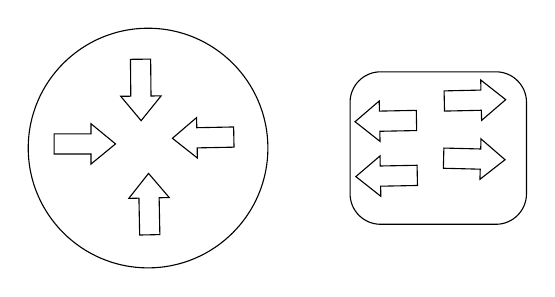
\begin{tikzpicture}[x=0.75pt, y=0.75pt, yscale=-1, xscale=1]
		%uncomment if require: \path (0,300); %set diagram left start at 0, and has height of 300

		%Shape: Circle [id:dp5361374648292709]
		\draw (34.54,160.73) .. controls (34.54,128.85) and (60.38,103) .. (92.27,103)
		.. controls (124.15,103) and (150,128.85) .. (150,160.73) .. controls (150,192.62)
		and (124.15,218.46) .. (92.27,218.46) .. controls (60.38,218.46) and (34.54,192.62)
		.. (34.54,160.73) -- cycle ;
		%Right Arrow [id:dp06422841843475346]
		\draw (47,153.87) -- (64.76,153.87) -- (64.76,149) -- (76.6,158.73) -- (64.76,168.46)
		-- (64.76,163.6) -- (47,163.6) -- cycle ;
		%Right Arrow [id:dp6209855052918765]
		\draw (133.69,160.3) -- (115.94,160.65) -- (116.03,165.52) -- (104,156.03) --
		(115.65,146.06) -- (115.74,150.93) -- (133.5,150.57) -- cycle ;
		%Right Arrow [id:dp5317728353939126]
		\draw (88.23,202.63) -- (87.88,184.87) -- (83.01,184.97) -- (92.51,172.93) --
		(102.47,184.58) -- (97.61,184.68) -- (97.96,202.43) -- cycle ;
		%Right Arrow [id:dp6187687437252627]
		\draw (93.52,117.88) -- (93.69,135.64) -- (98.56,135.6) -- (88.94,147.53) --
		(79.1,135.79) -- (83.96,135.74) -- (83.79,117.98) -- cycle ;
		%Rounded Rect [id:dp1889585755540648]
		\draw (189.6,138.69) .. controls (189.6,130.58) and (196.18,124) .. (204.29,124)
		-- (259.91,124) .. controls (268.02,124) and (274.6,130.58) .. (274.6,138.69)
		-- (274.6,182.77) .. controls (274.6,190.88) and (268.02,197.46) .. (259.91,197.46)
		-- (204.29,197.46) .. controls (196.18,197.46) and (189.6,190.88) .. (189.6,182.77)
		-- cycle ;
		%Right Arrow [id:dp7169185378424765]
		\draw (221.69,152.3) -- (203.94,152.65) -- (204.03,157.52) -- (192,148.03) --
		(203.65,138.06) -- (203.74,142.93) -- (221.5,142.57) -- cycle ;
		%Right Arrow [id:dp5328960964502949]
		\draw (222.08,178.76) -- (204.32,179.11) -- (204.42,183.98) -- (192.39,174.48)
		-- (204.03,164.52) -- (204.13,169.38) -- (221.89,169.03) -- cycle ;
		%Right Arrow [id:dp7192082508077764]
		\draw (234.8,160.73) -- (252.55,161.18) -- (252.68,156.32) -- (264.27,166.35)
		-- (252.18,175.78) -- (252.31,170.91) -- (234.55,170.46) -- cycle ;
		%Right Arrow [id:dp4880205307308063]
		\draw (234.9,133.19) -- (252.65,132.8) -- (252.55,127.94) -- (264.6,137.41) --
		(252.97,147.4) -- (252.86,142.53) -- (235.11,142.92) -- cycle ;
	\end{tikzpicture}

	Two PCs connected with eachother is called networks.Now that they are connected
	with eachother they can share the data with eachother. \textbf{Client}\\ A
	Client is a device that accesses a service available by a server. \\ \textbf{Server}\\
	A device that provides function or services for clients. A server can also be
	a client. \nt{The same device can be a client in some situations, and a server in other situations.}
	Typically you don't connect PCs or severs directly to eachother. You aggregate
	the connections to a device called a switch. Switches have a lot of interfaces
	for you to connect end hosts to. Switches are used to forward netork with a LAN
	a local area network. We have one LAN on the left and one LAN ont the right. The
	hosts within each LAN(such as network printer, pcs) can send data from one another.
	for example PC1 and PC2. These switches cannot cannot with eachother.\\
	\begin{itemize}
		\item have many network interfaces/ports for end hosts to connect to (usually
			24+).

		\item provide connectivity to hosts with the same LAN.

		\item donot provide connectivity between LANS/over the internet. We need
			another type of device called router.
	\end{itemize}
	\textbf{Router} \\ When end hosts in the New York Branch LAN want to
	communicate with end hosts in the Tokyo branch LAN , they will send the data
	to their router R1, which will then forward the data to the Tokyo Branch via internet.\\
	So, lets suppose a scenario when the PC in LAN1 wants a data from server1 of
	tokyo branch. It will request the data via a switch S1 which inturn connect with
	the router R1 and that router connects with the internet and the router R2 via
	switch S2 which connects the server and the data flow in the reverse order.\\ Types
	of Router\\
	\begin{itemize}
		\item ISR 1000

		\item ISR 900

		\item ISR 4000
	\end{itemize}
	% \begin{itemize}
	%     \item
	% \end{itemize}
	\textbf{Firewall}\\ Firewall are specially network security that controls
	network traffic entering an exiting your network. Firewalls can be placed 'outside'
	of your router.\\
	\begin{itemize}
		\item monitor and control network traffic based on configured rules

		\item can be placed inside the network or outside the network.

		\item are known as 'Next-Generation Firewalls when thry include more modern
			and advanced filtering capabilties.
	\end{itemize}
	What about the firewall on your computer?\\
	% Types of Firewalls\\
	\textbf{Types of switches}
	\textbf{Layer2 Swtich}
	A layer 2 switch operates in layer 2 of OSI Model.Layer (data link) deals with MAC address. 
	When devices connect to layer 2 switch,it stores the MAC address in the Switch table .
	\textbf{Layer 3 Swtich or Multilayer Switch}
	It operates at layer 3 of the OSI model. It deals with the IP address It also operates at the layer 2 which works in MAC address

	\begin{itemize}
	Catalyst 9200 \nt{RJ = Registered Jack}
	\end{itemize}
	\textbf{Ethernet}\\ \textbf{Bits and bytes}\\ Bits : Series of 0's or 1's. When
	communicating across a copper network cable,a variation of the electrical signal
	is assumed as 0's or 1's. \\ Bytes: Series of 8 0's and 1's. \\ Speed is
	measured in bits per second.(Kbps,Mbps,Gbps,etc not bytes per second.) in Harddisk
	data is transmitted in the bytes per second. \textbf{Ethernet Standards}\\
	defined in IEEE 802.3 standard in 1983.
	\begin{itemize}
		\item 10Mbps Ethernet 10BASE-T\\

		\item 1000Mbps Fast Ethernet 100BASE-T\\

		\item 1Gbps Gigabit Ethernet 1000BASE-T\\

		\item 10Gbps 10 Gig Ethernet 10GBASE-T\\
	\end{itemize}
	\textbf{UTP cables } Unshielded Twisted Pair : Un shieled means that the wires
	have no metallic shield which can make them vulnerable to electrical interferences.
	The twist actually helps protect against electromagentic interference or EMI. Four
	pairs of wires twisted with each other.\\ 10BASE-T ans 100BASE-T = 2 pairs (4
	wires)\\ 1000BASE-T ans 1GBASE-T = 4 pairs (8 wires)\\ Routers transmits data on
	pin 1 and 2 and receive data on pins 3 and 6(this are same in PCs) but switch
	is exactly opposite.\\ Communication in between the routers donot work in this
	case .\\ \textbf{StraightThrough cable}\\ A straight through cable connects pin1
	to pin1 ,pin2 to pin2,pin3 to pin3 and etc.\\ \textbf{Crosscable cable}\\ Pin1
	connects to pin 3 and Pin2 connects to Pin 6 on the other end and Pin3
	connects to pin1 and Pin 6 connects to pin 2 on the left side.\\ \textbf{Auto
	MDI X}\\ Auto MDI X allows devices to automatically detect which pins their
	neighbour is transmitting data on and then adjust themselves to receive data
	on the other pins.\\

	\textbf{How to connect to a cisco device(console) }\\ Router\> = user EXEC
	mode \\ Router\# = privileged EXEC mode \\ Router(config)\# = Global configuration
	mode \\ Router\>enable = used to enter privileged EXEC mode \\ Router\#configure
	terminal = used to enter global configuration mode \\ Router(config)\# enable password
	<password>= configures a password to protect privileged exec mode\\ Router(config)\#
	service password -encryption = encrypts the enable password \\ Router(config)\#
	enable secret <password> = configures a more secure ,always -encypted enable
	password\\ Router(config) \# run privleged -exec level command from global configuration
	mode \\ Router(config) \#no command = removes the command\\ Router(config) \#show
	running-config = displays the current ,a ctive configuration file \\ Router(config)
	\#show startup-config = displays the saved confiuration file which will be loaded
	if the device is restarted \\ Router(config) \#write = saves the configuration
	\\ Router(config) \# write memory = saves the configuration \\ \textbf{Ethernet
	Frame}\\
	\begin{itemize}
		\item The minimum size for an Ethernet frame (Header + Payload + trailer)is
			64 bytes.

		\item 64bytes -18(header + trailer size )= 46 bytes

		\item therefore the minimum payload is less than 46 bytes .

		\item if the payload is less than 46 bytes , padding bytes are added.
	\end{itemize}
	\textbf{Mac Address}\\ 6 byte (48) bit physical address that is assigned to
	the device when the device is made. AKA burned in address. The mac address is
	globally unique.\\ The first 3 byte are the OUI (organizational unique identifier)
	which is assigned to the company making the device.\\ \nt{Unicast Frame\\ The frame that is destined for only one single target.\\ Unknown unicast frame = flood to all other interfaces except the one which sent it. }
	\nt{Dynamic or dynamically learned mac address are removed. The mac address are removed after five minutes of inactivity}
	\textbf{ARP}
	\begin{itemize}
		\item ARP stands for 'Address Resolution Protocol'

		\item ARp is used to discover the layer 2 address (MAC address) of a known IP
			address

		\item ARP request is unknown unicast frame

		\item ARP request is unicast frame
	\end{itemize}

	\textbf{Network Layer}
	\begin{itemize}
		\item Provides connectivity between different end hosts on different networks
			(i.e outside the network ).

		\item Provides logical addressing

		\item Provides path selection between sources and destination addresses

		\item Routers operate at Layer 3
	\end{itemize}

	\textbf{IPv4 Addressing}\\ The IP address is written in dotted decimal.It is
	splitted into four octets and then written in dotted decimal for our easiness.
	Since IP address is of 32 bits from which first 24 bits specify network portion
	and remaining 8 bytes specify hosts address.\\ So 192.168.1.254/24 means 192.168.1
	represent network portion and 254 represent host portion.\\ \textbf{Loop back
	Address }
	\begin{itemize}
		\item Address range 127.0.0.0-127.255.255.255.

		\item Used to test the network stack on the local device.
	\end{itemize}
	\textbf{TTL(Time to Live)} \\ In practice, indicates a 'hopcount ': each packet
	arrives at a router,the router decreases TTL by 1.\\
	\begin{itemize}
		\item Value of 6 :TCP

		\item Value of 17 :UDP

		\item Value of 1 :ICMP

		\item Value of 89 :OCPF(dynamic routing protocol)
	\end{itemize}
	\textbf{Routing Fundamentals} \\ Routing is the process that routers use to determine
	the path that IP packets should take over a network to reach theri destination.
	\begin{itemize}
		\item WHen routers receive packets, they look in the routing table to find
			the best route to forward that packet.

		\item Routers store routes to all of their known destinations ina routing table.
	\end{itemize}
	A route tells the router : to send a packet to destination X you should send
	the packet to next hop Y \\ or if the setination is directly connected to the
	touter ,send the packet directly to the destination\\ or if the destination is
	the routers own IP address receive the packet dor yourself(dont forward it) When
	you configure an IP address on an interface and enable the interface , two routes
	are automatically added to the routing table Connected route A route to the network
	connected to the internet\\ i.e if the interface' IP is 192.168.1.1/24 the route
	will be to 192.168.1.0/24\\ Tells the router "To send a packet to a destination
	in this network, send it out of the interface specified in the route\\ Local route
	A route to the exact IP address configured in the interface. If the router
	receive a packet and it doesnot have a route that matches the packet
	destination it will drop the packet.\\ \textbf{The Life of a packet} \\ The source
	is 192.168.1.1 pc1's ip address and the destination is 192.168.4.1 pc4's ip address.
	because pc1's ip address is in the range of 192.168.1.1 so it notices that the
	the ip address 192.168.4.1 is in a different network so it knows that it needs
	to send the packet to its default gateway which is R1. SO it is necessary for ARP
	request to find the mac of destination, So it will send a broadcast to all the
	interfaces of the switch S1 except the one that sent.

	\chapter{Subnetting}
	\section{CIDR(Classless Inter-Domain Routing)}
	IANA assignes IPv4 addresses/network to company based on their size. Howerver,
	this leads to wastage of IPs.
	\section{Subnet Mask}

	\chapter{VLANS}
	\section{Introduction}
	VLANs are configured on switches on a per interface basis.They logically
	separate end hosts at Layer 2. \\ Switches don't forward traffic directly
	between hosts in different VLANS as well as in same VLANS. \\ Lots of unnecessary
	broadcast traffic can reduce network performance.\\ Even within the same office
	you want to limit who has access to what. You can apply security policies on a
	router/firewall. because this is one LAN ,PCs can reach each other directly
	without traffic passing through the router.\\ So, even if you configure security
	policies,they won't have any effect A switch willn't forward traffic between VLANs,
	including broadcast/unknown unicast traffic.\\ Vlans 1,1002-1005 exists by
	default and cannot be deleted.\\ Although we separated the three departments
	into three subnets (layer3) they are still in the same broadcast domain (Layer
	2).\\ The router is used to route between VLANs. The switch does not perform inter
	VLAN routing.\\ VLANs logically separate end hosts at Layer 2.\\ An access
	port is a switch port which belongs to a single VLAN and usually connects to
	end hosts like PCs.It gives end host access to internet.\\ Switch Ports which
	carry multiple VLANs are called trunk ports.
	\begin{itemize}
		\item interface range g2/0 -2

		\item switchport mode access

		\item switchport access vlan 20

		\item Access VLAN doesn'ot exist. Creating Vlan 10
	\end{itemize}
	\begin{itemize}
		\item interface range g3/0 -3

		\item switchport mode access

		\item switchport access vlan 30

		\item Access VLAN doesn't exist. Creating Vlan 10
	\end{itemize}
	\section{Trunk Ports}
	\textbf{What is trunk ports or Tagged Port?}\\ The Switches will tag all
	frames that they send over a trunk link. This allow the receiving switch to know
	which VLAN the frame belongs to. IEEE 802.1Q is an industry standard protocol created
	by IEEE. The 802.1Q tag is inserted between the source and type/length fields of
	the ethernet header which is of length 32 bits. VID Vlan id identies the vlan
	the frame belongs to . 12 bits in length = 4096 total vlans range of 0-4095
	Vlan 0 and 4095 are reserved and can't be used.\\ The range of VLANs (1-4094)
	is divided into two sections
	\begin{itemize}
		\item Normal VLANs 1-1005

		\item Extended VLANs 1005-4094
	\end{itemize}
	A standard layer 2 switch will only forward traffic in the same VLAN. IT will not
	forward traffics betwenn VLANs.\\
        
        


	\section{SVI Switch Virtutal Interface}
	Multi layer Switch or Layer 3 switches

	\section{router on a stick (RAOS)}

	\chapter{LAN}
	It is the connection within the network where internet cannot be accessed.

	\section{2 Tier LAN architecture}
	The two tier LAN design consists of two hierachical layers:
	\begin{itemize}
		\item Access Layer

		\item Distribution Layer
	\end{itemize}

	Also called a Collapsed Core design because it omits a layer that is found in the
	Three tier design :the Core layer \textbf{Access Layer}
	\begin{itemize}
		\item the layer that end hosts connect to (PCs printers,camers,etc.)

		\item typically access layer switches have lots of ports for end hosts to connect
			to

		\item WoS marking is typically dine her

		\item Security services like port security, DAI are typically performed here.
	\end{itemize}

	\textbf{Distribution Layer}
	\begin{itemize}
		\item aggregates connections from the access layer switches

		\item typically is the border between layer 2 and layer 3
	\end{itemize}
	The distribution layer uses OSPF protocol and access layer uses the spanning tree
	protocol The access layer connects to the distribution layer switches are Layer
	2 connections, and then end hosts use the SVIs on the distribution layer
	switches as their default gateways. The distribution layer is used to connect to
	services such as Internet, WAN, etc.

	\begin{figure}
		\centering
		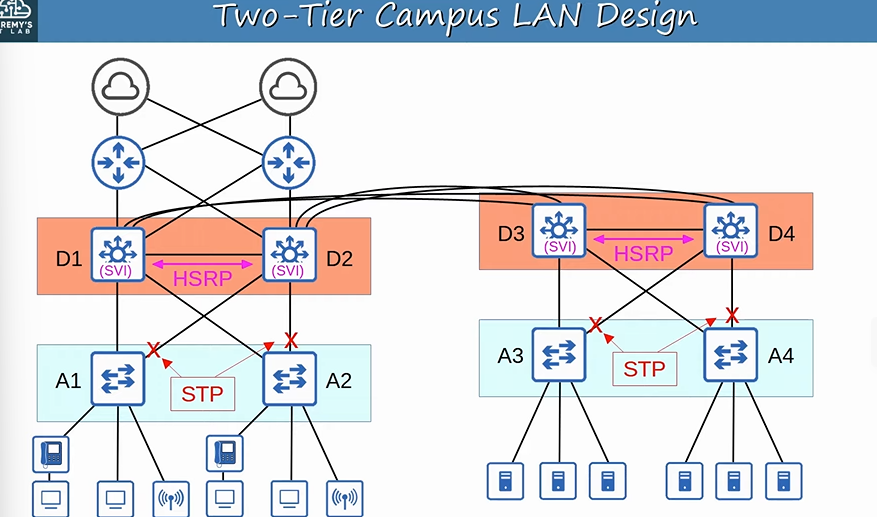
\includegraphics[width=0.5\linewidth]{image.png}
		\caption{2 Tier LAN}
		\label{fig:enter-label}
	\end{figure}
	\begin{figure}
		\centering
		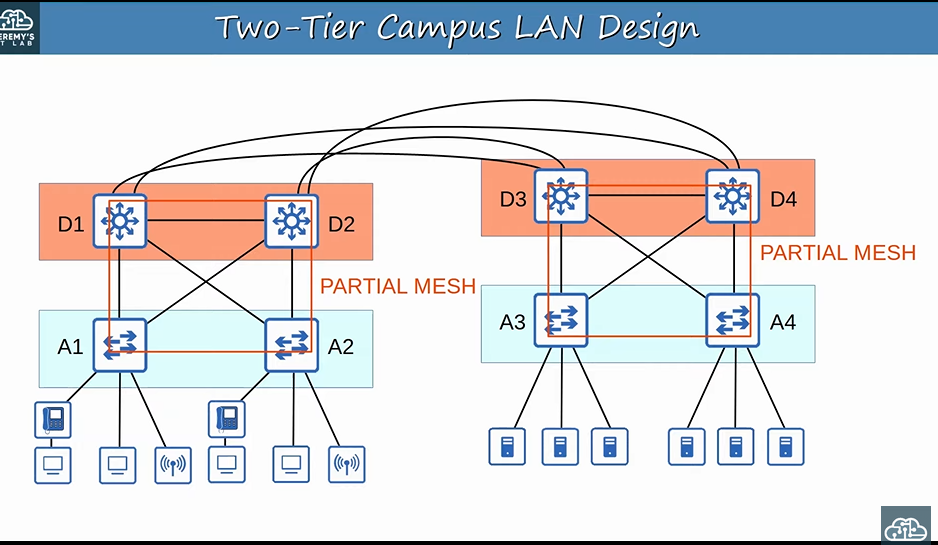
\includegraphics[width=0.5\linewidth]{2tier.png}
		\caption{2 tier LAN}
		\label{fig:enter-label}
	\end{figure}
	Connections between Distribution Switches are Layer 3. Routing information can
	be shared via OSPF for example In large LAN networks with many Distribution Layer
	switches(for example in separate buildings) the number of connection required
	between Distribution Layer switches grows rapidly.

	\section{3 Tier LAN architecture}
	The three tier LAN design consists of three hierarchical layers.
	\begin{figure}
		\centering
		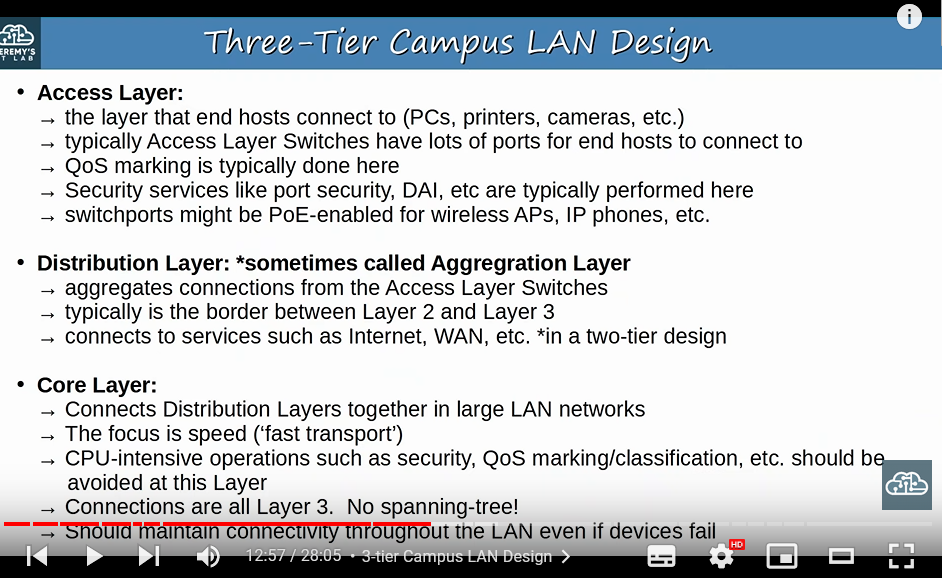
\includegraphics[width=0.5\linewidth]{3tierlan.png}
		\caption{Enter Caption}
		\label{fig:enter-label}
	\end{figure}
	\begin{figure}
		\centering
		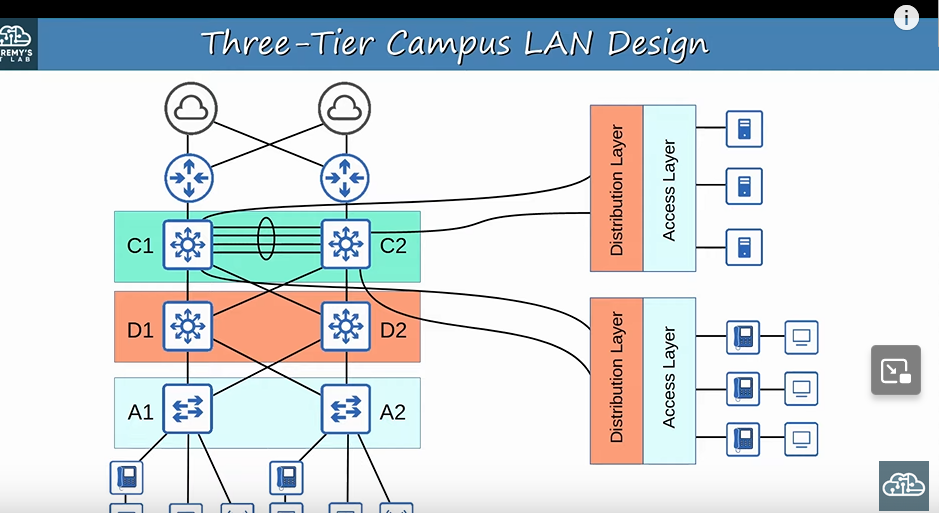
\includegraphics[width=0.5\linewidth]{3tierlan1.png}
		\caption{Enter Caption}
		\label{fig:enter-label}
	\end{figure}

	\section{Spine Leaf Architecture}
	IT is used in data center. Data centers are dedicated spaces/buildings used to
	store computer systems such as servers and network devices. Traditional Data
	center designs used a three tier architecture like we just covered. This worked
	well when most traffic in the data center was North-South. With the precedence
	of virtual servers, applications are oftern deployed in a distributed manner(across
	multiple physical servers) which increases the amount of East-West traffic in
	the data center.The traditional design led to the bottleneck in bandwidth and
	speed. There are spine switches and leaf switches, and here are the basic
	rules about spine-leaf architecture. Every leaf switch is connected to every spine
	switch. If you look at the diagram below, there are three spine switches, and
	each leaf switch has three uplinks, one to each spine switch. Therefore, every
	spine switch is connected to every leaf switch too. However, leaf switches do not
	connect to other leaf switches, and spine switches do not connect to other
	spine switches. Finally, end hosts, for example servers, only connect to leaf
	switches. They are like the ‘access layer’ of the spine-leaf architecture.
	\begin{figure}
		\centering
		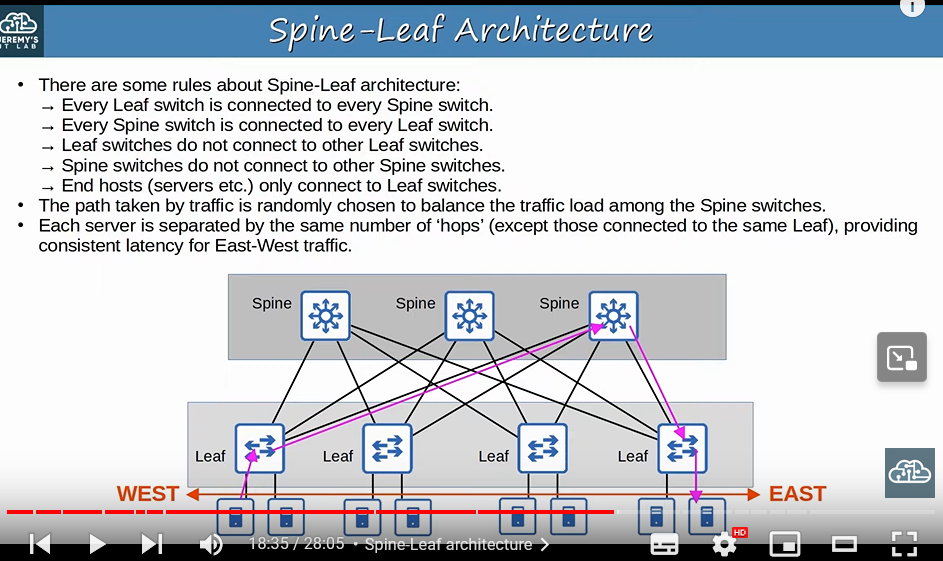
\includegraphics[width=0.5\linewidth]{spinceleaf.png}
		\caption{Enter Caption}
		\label{fig:enter-label}
	\end{figure}

	\section{SOHO Networks}

	Small office/Home Office (SOHO) refers ti the office of a small company or a
	small home office with the few devices. ->Does not have to be an actual home office,
	if your home has network connected to the internet considered a SOHO network. SOHO
	networks don't have complex needs so all networking functions are typically provided
	by a single device often called a home router or wireless router. This device
	can serve as a
	\begin{itemize}
		\item Router

		\item Switch

		\item Firewall

		\item Wireless access Point

		\item Modem
	\end{itemize}

	\chapter{Wireless LAN}

	\section{Wireless Lan Controller}
	It is an appliance which centralizes all the control of the access points. By
	using WLCs all management are transferred from APs to the WLCs such as
	authentication,and more. To change the config of APs WLC are used to use to change
	all at once.It can also provide the statistics and performance metrics. The
	APs then are called Lightweight APs which only handle the forwarding the
	traffic.

	\section{Wireless Architecture}

	\subsection{Wireless}
	\begin{itemize}
		\item It's possible for an AP to provide the multiple wireless LANS,each with
			unique SSIDs.

		\item Each WLAN is mapped to a separate VLAN and connected to the wired network
			via a trunk.

		\item Each WLAN uses a unique BSSID, usually by incrementing the last digit
			of the previous BSSID.
	\end{itemize}
	Additional AP operational Modes beyond one. An AP in repeater mode can be used
	to extend the range of a BSS. The repeater will simply re transmit any signal it
	receives from the AP. A repeater with a single radio must operate on the same
	channel as the AP.

	A workgroup bridge operates as a wireless client of another AP and can be used
	to connect wired devices to the wireless network.

	802.11 Frame Format

	Addresses: Up to four address can be present. Which addresses are present anf their
	order dependes on the message type.
	\begin{itemize}
		\item Destination Address: Final recipient of the frame.
	\end{itemize}
	\begin{itemize}
		\item Source address :Original sender if the frame

		\item Transmitter address Immediate sender of the frame

		\item Recipient frame: Immediate receiver of the frame.
	\end{itemize}

	Access Point bridge traffic between wireless stations and other devices. There
	are three 802.11 connection states.
	\begin{itemize}
		\item Not authenticated, not associated.

		\item Authenticated, not associated.

		\item Authenticated, associated.
	\end{itemize}

	\subsection{Lightweight APs}
	\begin{itemize}
		\item
	\end{itemize}
\end{document}